% Options for packages loaded elsewhere
\PassOptionsToPackage{unicode}{hyperref}
\PassOptionsToPackage{hyphens}{url}
\PassOptionsToPackage{dvipsnames,svgnames,x11names}{xcolor}
%
\documentclass[
  letterpaper,
  DIV=11,
  numbers=noendperiod]{scrartcl}

\usepackage{amsmath,amssymb}
\usepackage{iftex}
\ifPDFTeX
  \usepackage[T1]{fontenc}
  \usepackage[utf8]{inputenc}
  \usepackage{textcomp} % provide euro and other symbols
\else % if luatex or xetex
  \usepackage{unicode-math}
  \defaultfontfeatures{Scale=MatchLowercase}
  \defaultfontfeatures[\rmfamily]{Ligatures=TeX,Scale=1}
\fi
\usepackage{lmodern}
\ifPDFTeX\else  
    % xetex/luatex font selection
\fi
% Use upquote if available, for straight quotes in verbatim environments
\IfFileExists{upquote.sty}{\usepackage{upquote}}{}
\IfFileExists{microtype.sty}{% use microtype if available
  \usepackage[]{microtype}
  \UseMicrotypeSet[protrusion]{basicmath} % disable protrusion for tt fonts
}{}
\makeatletter
\@ifundefined{KOMAClassName}{% if non-KOMA class
  \IfFileExists{parskip.sty}{%
    \usepackage{parskip}
  }{% else
    \setlength{\parindent}{0pt}
    \setlength{\parskip}{6pt plus 2pt minus 1pt}}
}{% if KOMA class
  \KOMAoptions{parskip=half}}
\makeatother
\usepackage{xcolor}
\setlength{\emergencystretch}{3em} % prevent overfull lines
\setcounter{secnumdepth}{-\maxdimen} % remove section numbering
% Make \paragraph and \subparagraph free-standing
\makeatletter
\ifx\paragraph\undefined\else
  \let\oldparagraph\paragraph
  \renewcommand{\paragraph}{
    \@ifstar
      \xxxParagraphStar
      \xxxParagraphNoStar
  }
  \newcommand{\xxxParagraphStar}[1]{\oldparagraph*{#1}\mbox{}}
  \newcommand{\xxxParagraphNoStar}[1]{\oldparagraph{#1}\mbox{}}
\fi
\ifx\subparagraph\undefined\else
  \let\oldsubparagraph\subparagraph
  \renewcommand{\subparagraph}{
    \@ifstar
      \xxxSubParagraphStar
      \xxxSubParagraphNoStar
  }
  \newcommand{\xxxSubParagraphStar}[1]{\oldsubparagraph*{#1}\mbox{}}
  \newcommand{\xxxSubParagraphNoStar}[1]{\oldsubparagraph{#1}\mbox{}}
\fi
\makeatother


\providecommand{\tightlist}{%
  \setlength{\itemsep}{0pt}\setlength{\parskip}{0pt}}\usepackage{longtable,booktabs,array}
\usepackage{calc} % for calculating minipage widths
% Correct order of tables after \paragraph or \subparagraph
\usepackage{etoolbox}
\makeatletter
\patchcmd\longtable{\par}{\if@noskipsec\mbox{}\fi\par}{}{}
\makeatother
% Allow footnotes in longtable head/foot
\IfFileExists{footnotehyper.sty}{\usepackage{footnotehyper}}{\usepackage{footnote}}
\makesavenoteenv{longtable}
\usepackage{graphicx}
\makeatletter
\def\maxwidth{\ifdim\Gin@nat@width>\linewidth\linewidth\else\Gin@nat@width\fi}
\def\maxheight{\ifdim\Gin@nat@height>\textheight\textheight\else\Gin@nat@height\fi}
\makeatother
% Scale images if necessary, so that they will not overflow the page
% margins by default, and it is still possible to overwrite the defaults
% using explicit options in \includegraphics[width, height, ...]{}
\setkeys{Gin}{width=\maxwidth,height=\maxheight,keepaspectratio}
% Set default figure placement to htbp
\makeatletter
\def\fps@figure{htbp}
\makeatother

\usepackage{fvextra}
\DefineVerbatimEnvironment{Highlighting}{Verbatim}{breaklines,commandchars=\\\{\}}
\KOMAoption{captions}{tableheading}
\makeatletter
\@ifpackageloaded{caption}{}{\usepackage{caption}}
\AtBeginDocument{%
\ifdefined\contentsname
  \renewcommand*\contentsname{Table of contents}
\else
  \newcommand\contentsname{Table of contents}
\fi
\ifdefined\listfigurename
  \renewcommand*\listfigurename{List of Figures}
\else
  \newcommand\listfigurename{List of Figures}
\fi
\ifdefined\listtablename
  \renewcommand*\listtablename{List of Tables}
\else
  \newcommand\listtablename{List of Tables}
\fi
\ifdefined\figurename
  \renewcommand*\figurename{Figure}
\else
  \newcommand\figurename{Figure}
\fi
\ifdefined\tablename
  \renewcommand*\tablename{Table}
\else
  \newcommand\tablename{Table}
\fi
}
\@ifpackageloaded{float}{}{\usepackage{float}}
\floatstyle{ruled}
\@ifundefined{c@chapter}{\newfloat{codelisting}{h}{lop}}{\newfloat{codelisting}{h}{lop}[chapter]}
\floatname{codelisting}{Listing}
\newcommand*\listoflistings{\listof{codelisting}{List of Listings}}
\makeatother
\makeatletter
\makeatother
\makeatletter
\@ifpackageloaded{caption}{}{\usepackage{caption}}
\@ifpackageloaded{subcaption}{}{\usepackage{subcaption}}
\makeatother

\ifLuaTeX
  \usepackage{selnolig}  % disable illegal ligatures
\fi
\usepackage{bookmark}

\IfFileExists{xurl.sty}{\usepackage{xurl}}{} % add URL line breaks if available
\urlstyle{same} % disable monospaced font for URLs
\hypersetup{
  pdftitle={Final Project: Writeup},
  pdfauthor={Jae Hu (jianinghu0408), Duoshu Xu (KevinX0), Regina Hou (Reginahk), Section 3},
  colorlinks=true,
  linkcolor={blue},
  filecolor={Maroon},
  citecolor={Blue},
  urlcolor={Blue},
  pdfcreator={LaTeX via pandoc}}


\title{Final Project: Writeup}
\author{Jae Hu (jianinghu0408), Duoshu Xu (KevinX0), Regina Hou
(Reginahk), Section 3}
\date{}

\begin{document}
\maketitle

\RecustomVerbatimEnvironment{verbatim}{Verbatim}{
  showspaces = false,
  showtabs = false,
  breaksymbolleft={},
  breaklines
}


\begin{center}\rule{0.5\linewidth}{0.5pt}\end{center}

\section{Data cleaning and reshaping}\label{data-cleaning-and-reshaping}

\section{pie chart (done by Jae Hu)}\label{pie-chart-done-by-jae-hu}

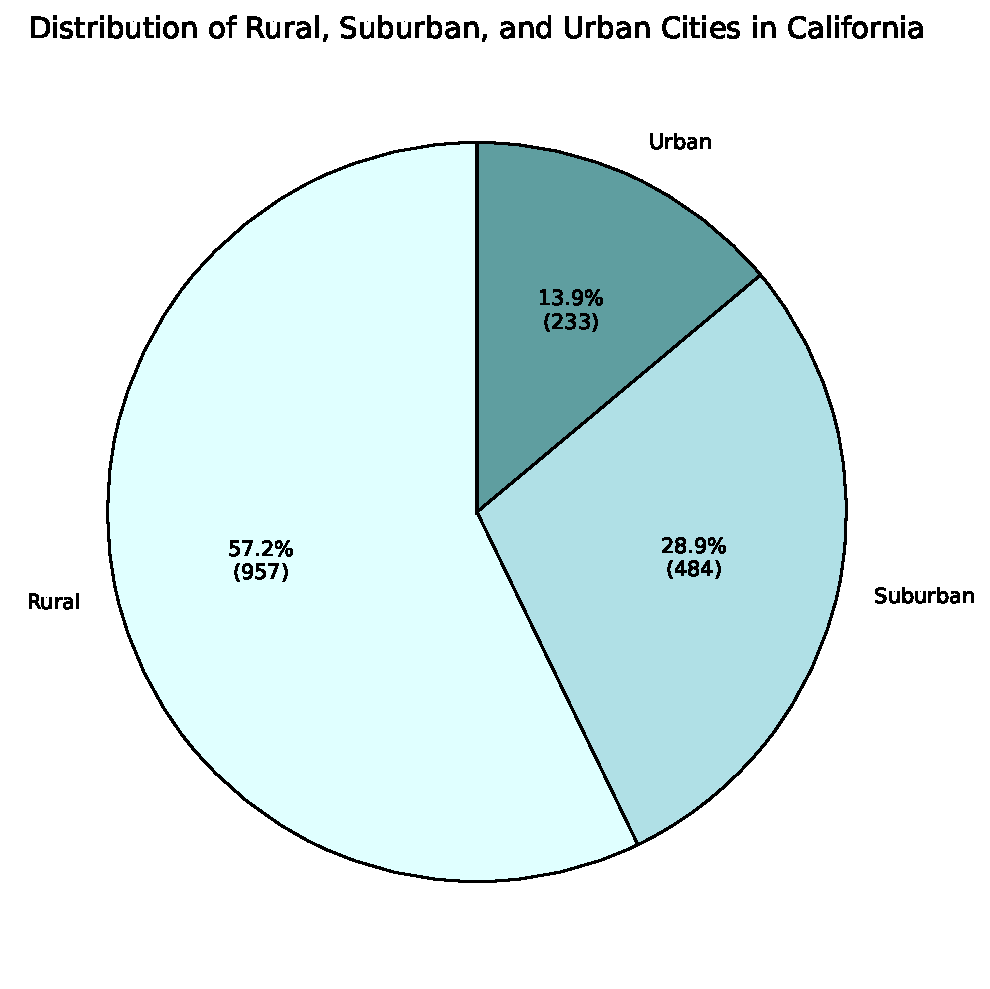
\includegraphics{Final Writeup_files/figure-pdf/cell-6-output-1.pdf}

\section{Wildfire Frequency bar chart (done by Duoshu
Xu)}\label{wildfire-frequency-bar-chart-done-by-duoshu-xu}

\begin{verbatim}
  Geographic Type  Number of Wildfires
0           Urban                 2356
1        Suburban                  407
2           Rural                   10
\end{verbatim}

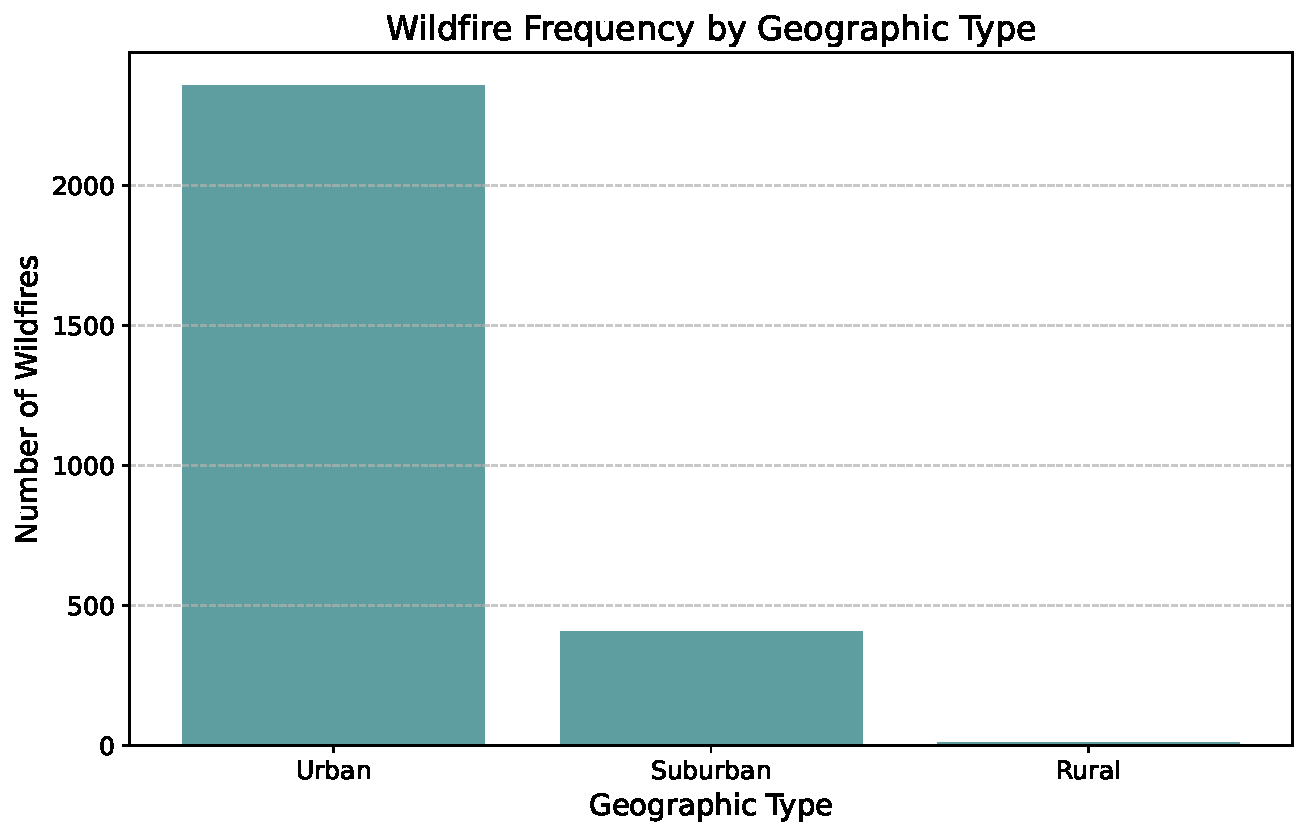
\includegraphics{Final Writeup_files/figure-pdf/cell-7-output-2.pdf}

\begin{verbatim}
['California' 'Alameda County' 'Alameda' 'Albany' 'Ashland CDP' 'Berkeley'
 'Castro Valley CDP' 'Cherryland CDP' 'Dublin' 'Emeryville']
\end{verbatim}

\begin{verbatim}
/var/folders/r4/x5b99tvj66zcn_88m3jn4r6w0000gn/T/ipykernel_23835/3288246651.py:4: DtypeWarning:

Columns (12,36) have mixed types. Specify dtype option on import or set low_memory=False.
\end{verbatim}

\begin{longtable}[]{@{}llllllll@{}}
\toprule\noalign{}
& Geography & Total Population & Land Area in Square Miles & Population
Per Square Mile (Land Area) & Unnamed: 4 & Geoid & geographic type \\
\midrule\noalign{}
\endhead
\bottomrule\noalign{}
\endlastfoot
0 & California & 39538223 & 155858.326771 & 253.680530 & NaN &
0400000US06 & Urban \\
1 & Alameda County & 1682353 & 737.461854 & 2281.274605 & NaN &
0500000US06001 & Urban \\
2 & Alameda & 78280 & 10.448679 & 7491.856487 & NaN & 1600000US0600562 &
Urban \\
3 & Albany & 20271 & 1.789982 & 11324.694641 & NaN & 1600000US0600674 &
Suburban \\
4 & Ashland CDP & 23823 & 1.842571 & 12929.213531 & NaN &
1600000US0602980 & Suburban \\
\end{longtable}

\begin{longtable}[]{@{}llllllllllllllllllllll@{}}
\toprule\noalign{}
& OBJECTID & * Damage & * Street Number & * Street Name & * Street Type
(e.g. road, drive, lane, etc.) & Street Suffix (e.g. apt. 23, blding C)
& * City & State & Zip Code & * CAL FIRE Unit & ... & Fire Name
(Secondary) & APN (parcel) & Assessed Improved Value (parcel) & Year
Built (parcel) & Site Address (parcel) & GLOBALID & Latitude & Longitude
& x & y \\
\midrule\noalign{}
\endhead
\bottomrule\noalign{}
\endlastfoot
0 & 1 & No Damage & 8376.0 & Quail Canyon & Road & NaN & Winters & CA &
NaN & LNU & ... & Quail & 101090290 & 510000.0 & 1997.0 & 8376 QUAIL
CANYON RD VACAVILLE CA 95688 & e1919a06-b4c6-476d-99e5-f0b45b070de8 &
38.474960 & -122.044465 & -1.358593e+07 & 4.646741e+06 \\
1 & 2 & Affected (1-9\%) & 8402.0 & Quail Canyon & Road & NaN & Winters
& CA & NaN & LNU & ... & Quail & 101090270 & 573052.0 & 1980.0 & 8402
QUAIL CANYON RD VACAVILLE CA 95688 &
b090eeb6-5b18-421e-9723-af7c9144587c & 38.477442 & -122.043252 &
-1.358579e+07 & 4.647094e+06 \\
2 & 3 & No Damage & 8430.0 & Quail Canyon & Road & NaN & Winters & CA &
NaN & LNU & ... & Quail & 101090310 & 350151.0 & 2004.0 & 8430 QUAIL
CANYON RD VACAVILLE CA 95688 & 268da70b-753f-46aa-8fb1-327099337395 &
38.479358 & -122.044585 & -1.358594e+07 & 4.647366e+06 \\
3 & 4 & No Damage & 3838.0 & Putah Creek & Road & NaN & Winters & CA &
NaN & LNU & ... & Quail & 103010240 & 134880.0 & 1981.0 & 3838 PUTAH
CREEK RD WINTERS CA 95694 & 64d4a278-5ee9-414a-8bf4-247c5b5c60f9 &
38.487313 & -122.015115 & -1.358266e+07 & 4.648497e+06 \\
4 & 5 & No Damage & 3830.0 & Putah Creek & Road & NaN & Winters & CA &
NaN & LNU & ... & Quail & 103010220 & 346648.0 & 1980.0 & 3830 PUTAH
CREEK RD WINTERS CA 95694 & 1b44b214-01fd-4f06-b764-eb42a1ec93d7 &
38.485636 & -122.016122 & -1.358277e+07 & 4.648259e+06 \\
\end{longtable}

\begin{longtable}[]{@{}llllllllllllllllllllll@{}}
\toprule\noalign{}
& OBJECTID & * Damage & * Street Number & * Street Name & * Street Type
(e.g. road, drive, lane, etc.) & Street Suffix (e.g. apt. 23, blding C)
& City & State & Zip Code & * CAL FIRE Unit & ... & Latitude & Longitude
& x & y & Total Population & Land Area in Square Miles & Population Per
Square Mile (Land Area) & Unnamed: 4 & Geoid & geographic type \\
\midrule\noalign{}
\endhead
\bottomrule\noalign{}
\endlastfoot
0 & 1 & No Damage & 8376.0 & Quail Canyon & Road & NaN & Winters & CA &
NaN & LNU & ... & 38.474960 & -122.044465 & -1.358593e+07 & 4.646741e+06
& 7115 & 2.934826 & 2424.334246 & NaN & 1600000US0686034 & Suburban \\
1 & 2 & Affected (1-9\%) & 8402.0 & Quail Canyon & Road & NaN & Winters
& CA & NaN & LNU & ... & 38.477442 & -122.043252 & -1.358579e+07 &
4.647094e+06 & 7115 & 2.934826 & 2424.334246 & NaN & 1600000US0686034 &
Suburban \\
2 & 3 & No Damage & 8430.0 & Quail Canyon & Road & NaN & Winters & CA &
NaN & LNU & ... & 38.479358 & -122.044585 & -1.358594e+07 & 4.647366e+06
& 7115 & 2.934826 & 2424.334246 & NaN & 1600000US0686034 & Suburban \\
3 & 4 & No Damage & 3838.0 & Putah Creek & Road & NaN & Winters & CA &
NaN & LNU & ... & 38.487313 & -122.015115 & -1.358266e+07 & 4.648497e+06
& 7115 & 2.934826 & 2424.334246 & NaN & 1600000US0686034 & Suburban \\
4 & 5 & No Damage & 3830.0 & Putah Creek & Road & NaN & Winters & CA &
NaN & LNU & ... & 38.485636 & -122.016122 & -1.358277e+07 & 4.648259e+06
& 7115 & 2.934826 & 2424.334246 & NaN & 1600000US0686034 & Suburban \\
\end{longtable}

\section{bar plot of 2020 (done by Regina
Hou)}\label{bar-plot-of-2020-done-by-regina-hou}

\begin{verbatim}
/var/folders/r4/x5b99tvj66zcn_88m3jn4r6w0000gn/T/ipykernel_23835/454140121.py:2: UserWarning:

Could not infer format, so each element will be parsed individually, falling back to `dateutil`. To ensure parsing is consistent and as-expected, please specify a format.
\end{verbatim}

\begin{verbatim}
/var/folders/r4/x5b99tvj66zcn_88m3jn4r6w0000gn/T/ipykernel_23835/3001088990.py:3: UserWarning:

Could not infer format, so each element will be parsed individually, falling back to `dateutil`. To ensure parsing is consistent and as-expected, please specify a format.
\end{verbatim}

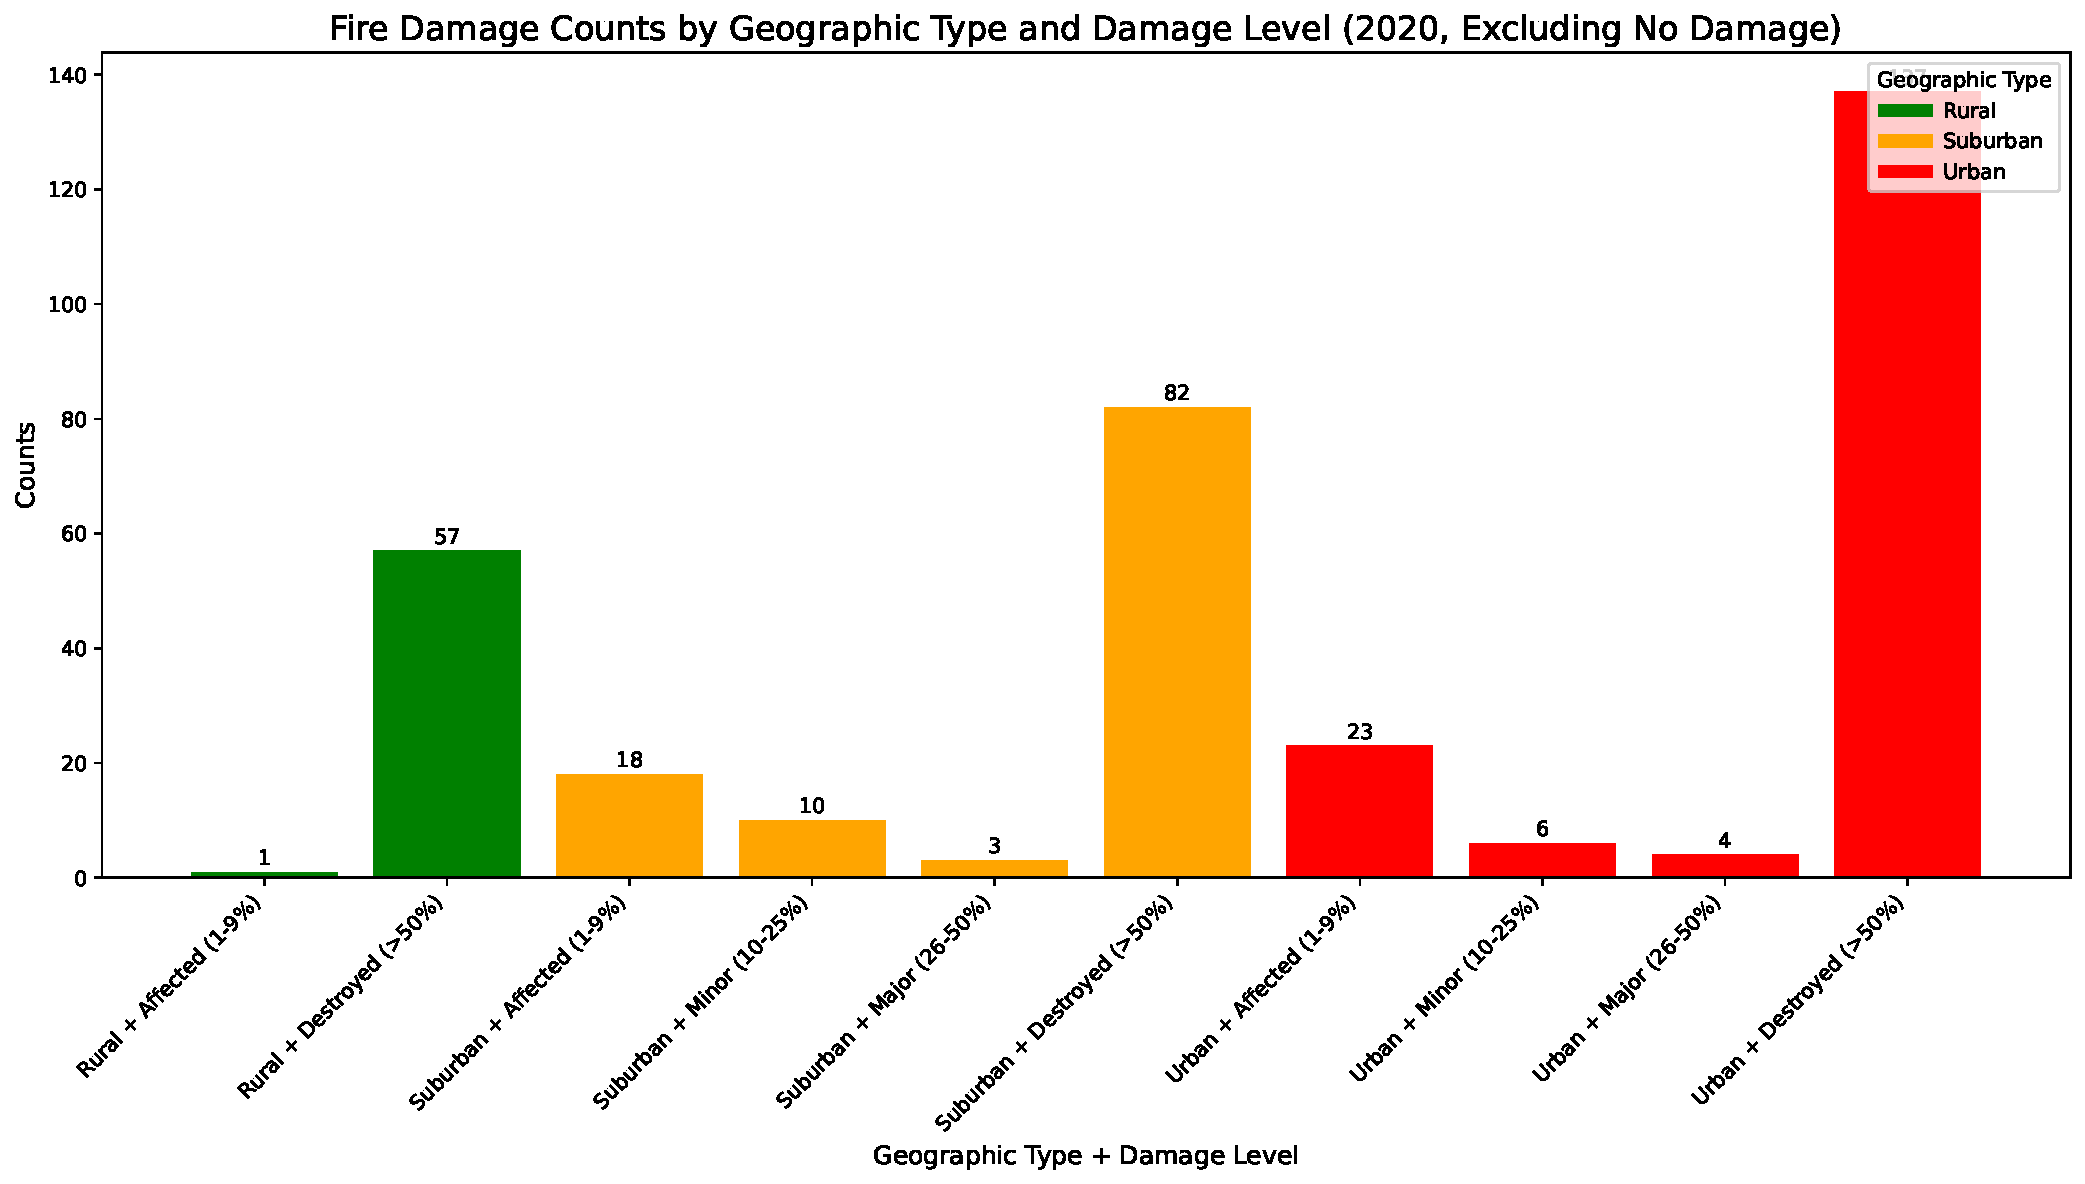
\includegraphics{Final Writeup_files/figure-pdf/cell-12-output-2.pdf}

\section{plot of 2021 (done by Regina
Hou)}\label{plot-of-2021-done-by-regina-hou}

\begin{verbatim}
NaN values in geographic type: 0
NaN values in * Damage: 0
\end{verbatim}

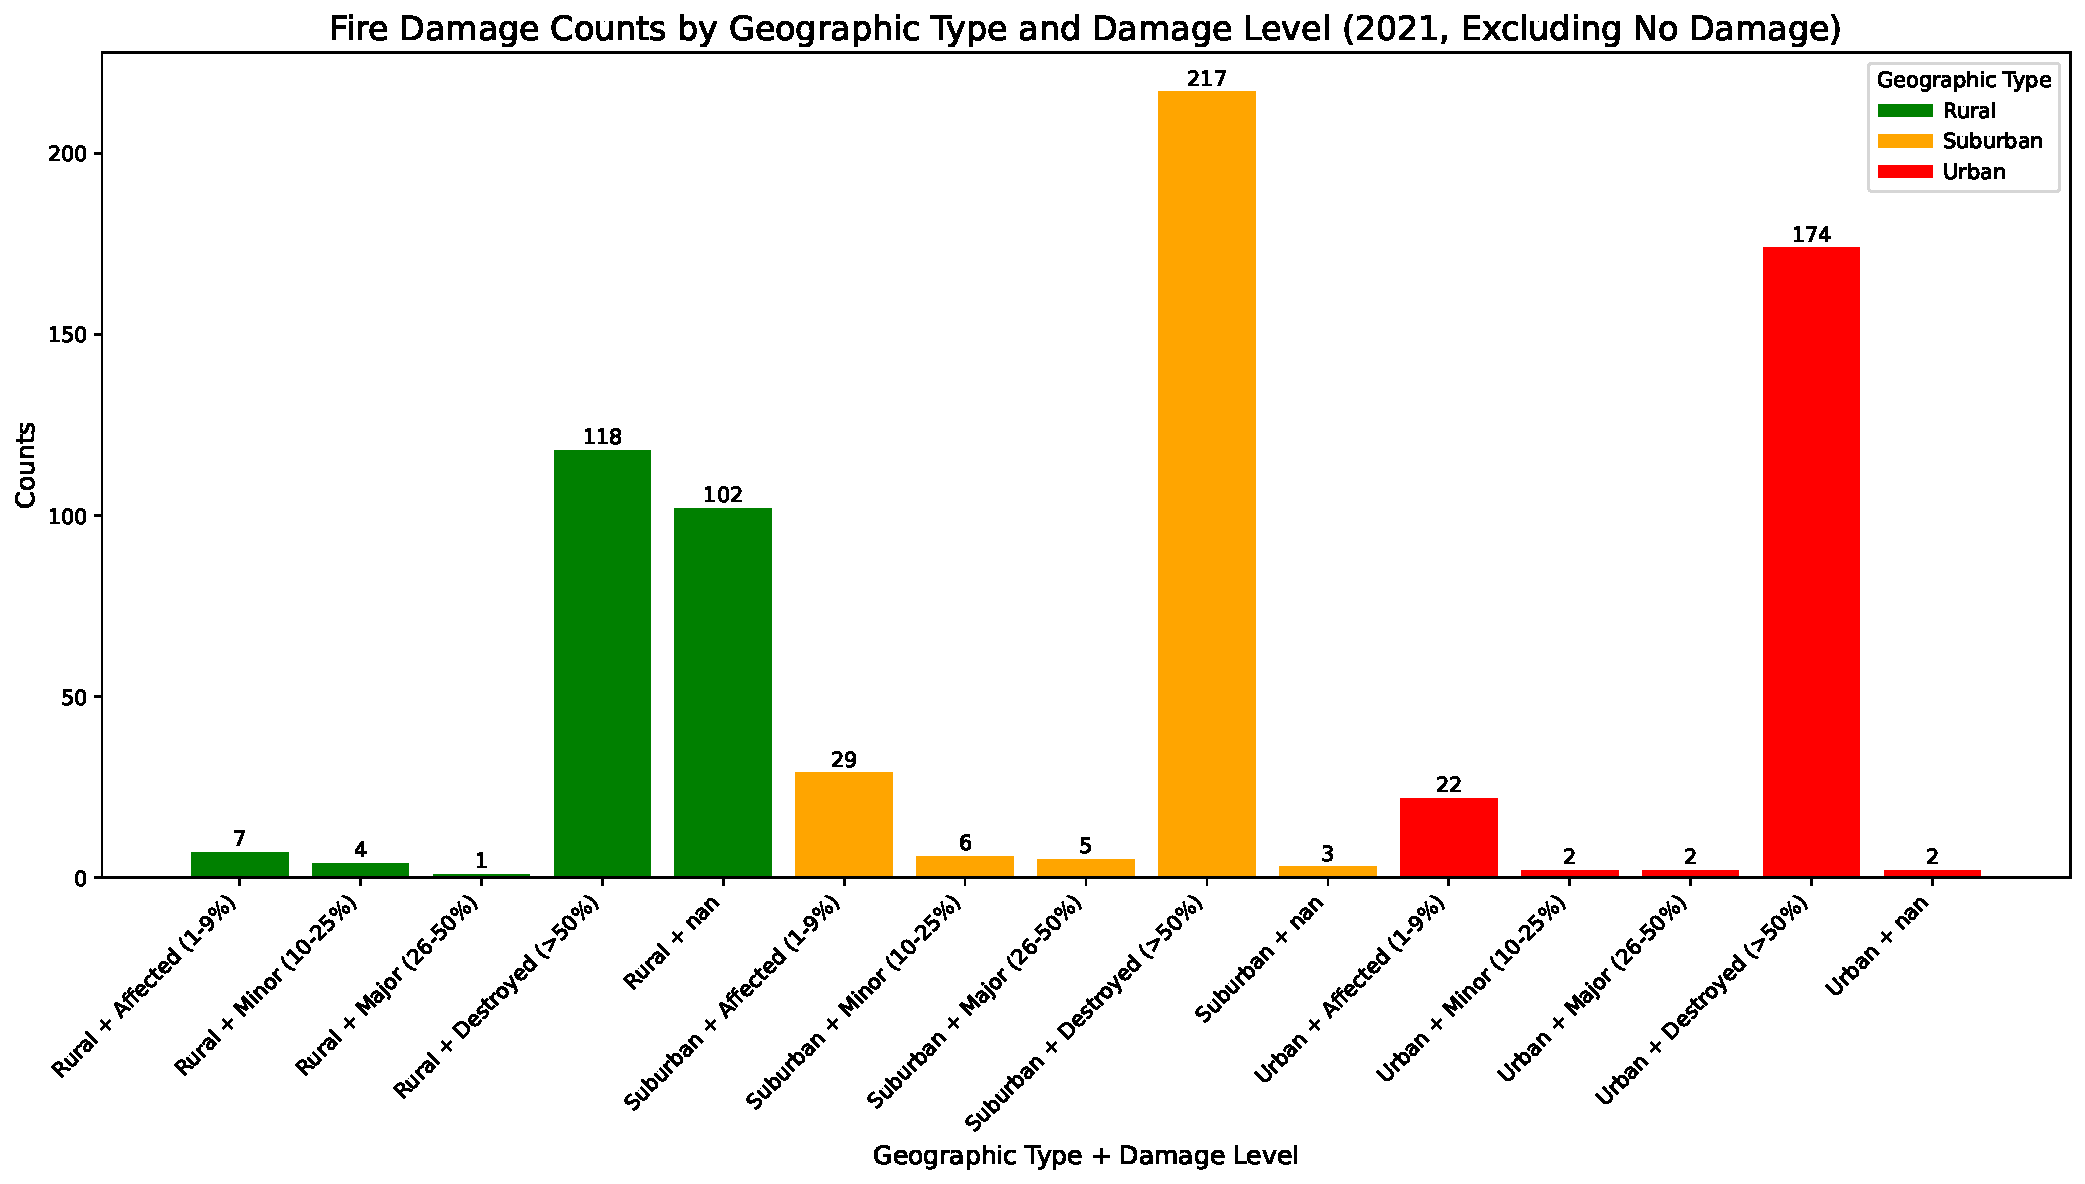
\includegraphics{Final Writeup_files/figure-pdf/cell-14-output-1.pdf}

\section{plot of 2022 (done by Regina
Hou)}\label{plot-of-2022-done-by-regina-hou}

\begin{verbatim}
/var/folders/r4/x5b99tvj66zcn_88m3jn4r6w0000gn/T/ipykernel_23835/3282159924.py:2: UserWarning:

Could not infer format, so each element will be parsed individually, falling back to `dateutil`. To ensure parsing is consistent and as-expected, please specify a format.
\end{verbatim}

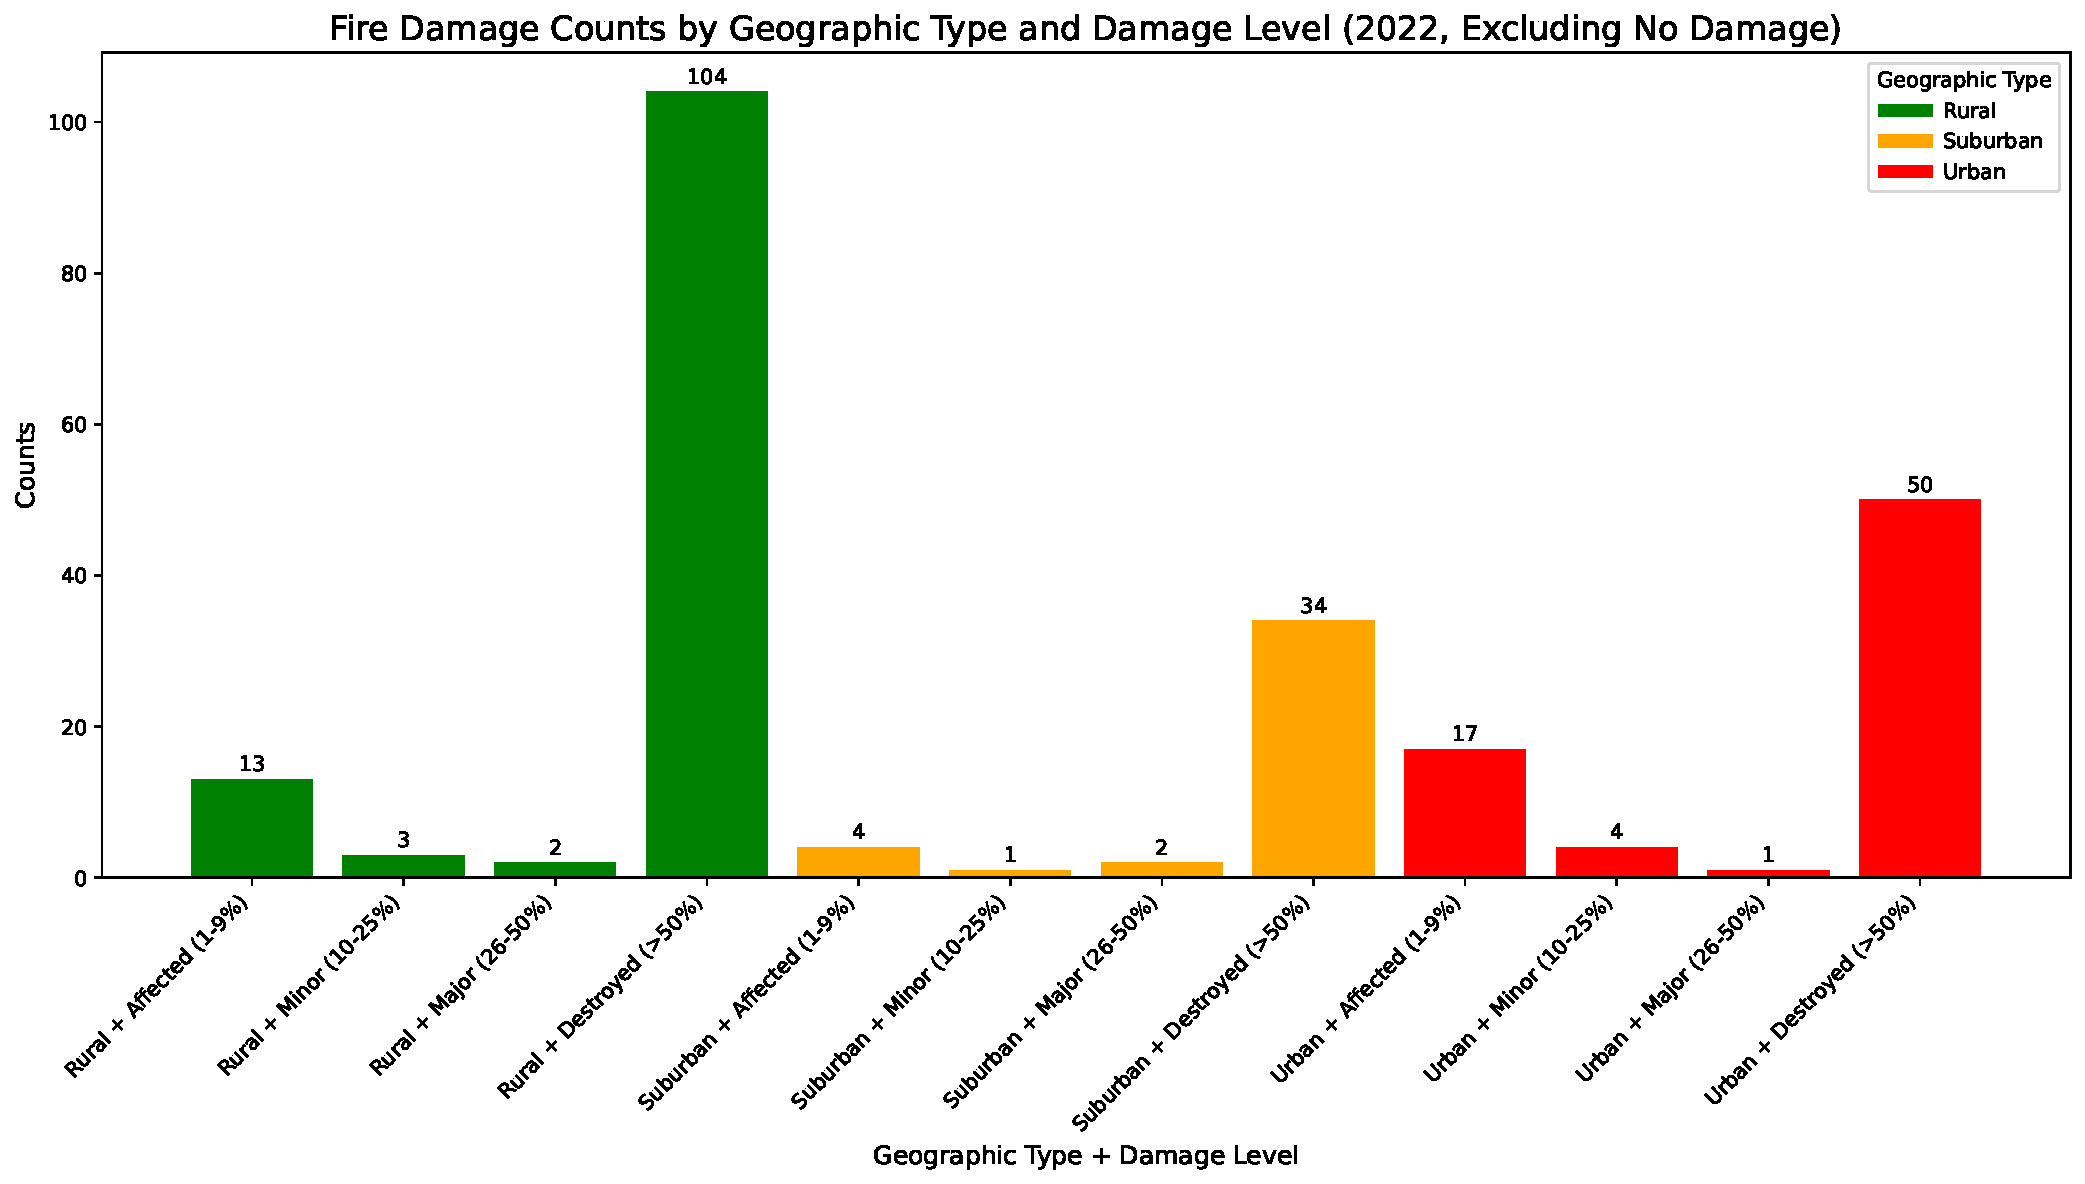
\includegraphics{Final Writeup_files/figure-pdf/cell-16-output-1.pdf}

\section{plot of 2023 (done by Regina
Hou)}\label{plot-of-2023-done-by-regina-hou}

\begin{verbatim}
/var/folders/r4/x5b99tvj66zcn_88m3jn4r6w0000gn/T/ipykernel_23835/897568859.py:2: UserWarning:

Could not infer format, so each element will be parsed individually, falling back to `dateutil`. To ensure parsing is consistent and as-expected, please specify a format.
\end{verbatim}

\section{plot for 2020-2023 (done by Regina
Hou)}\label{plot-for-2020-2023-done-by-regina-hou}

\begin{verbatim}
/var/folders/r4/x5b99tvj66zcn_88m3jn4r6w0000gn/T/ipykernel_23835/857330891.py:1: UserWarning:

Could not infer format, so each element will be parsed individually, falling back to `dateutil`. To ensure parsing is consistent and as-expected, please specify a format.
\end{verbatim}

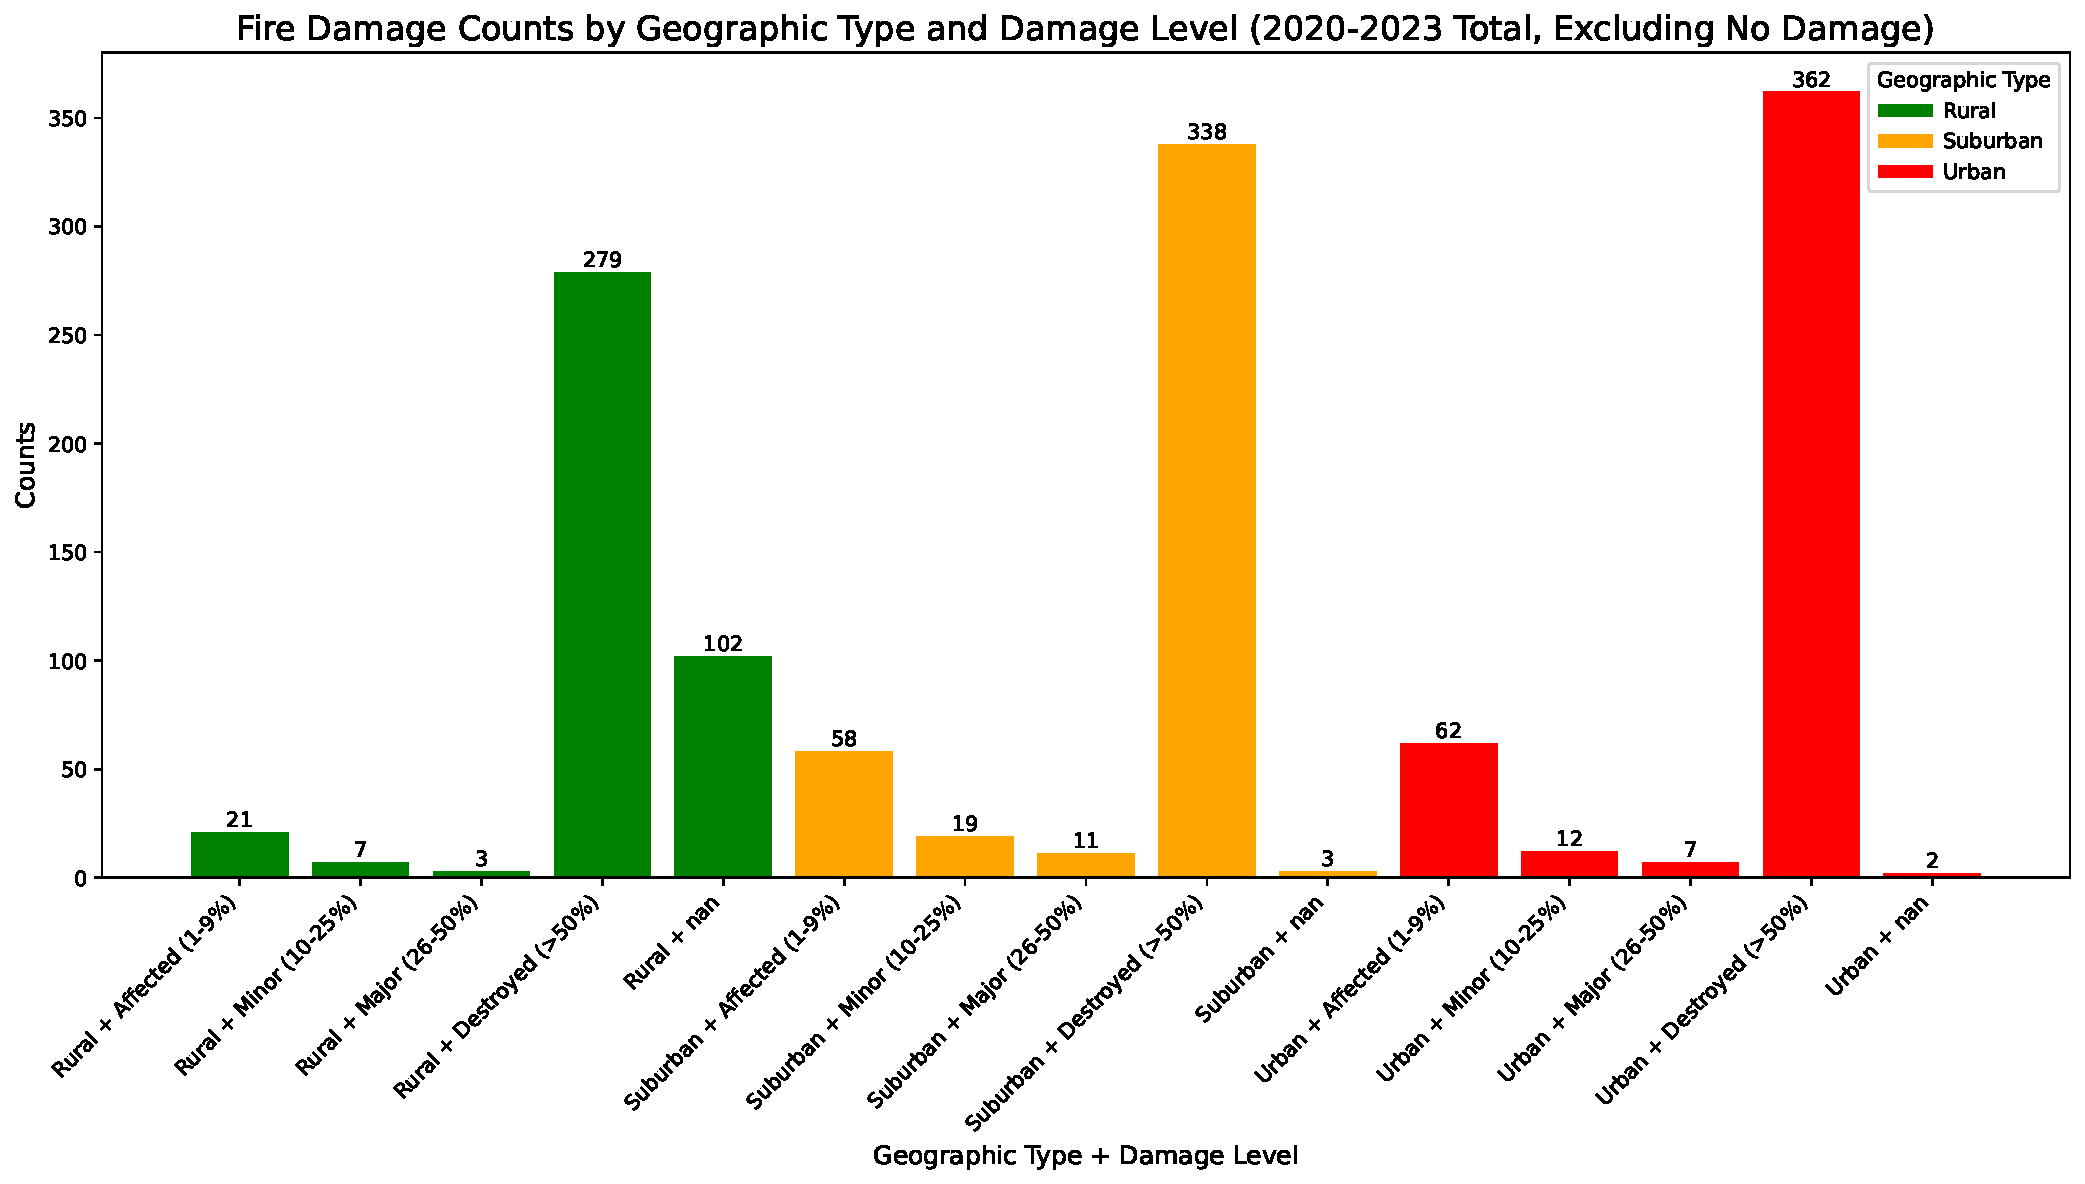
\includegraphics{Final Writeup_files/figure-pdf/cell-19-output-1.pdf}

Intro Wildfires are among the most destructive natural disasters in the
U.S., with California experiencing the greatest impact. In 2021, the
state accounted for 40\% of all burned acres nationwide and had nearly
two million properties at risk of wildfire damage---three times more
than the next highest state. The rising frequency and severity of
wildfires, driven by climate change, droughts, and urban expansion into
fire-prone areas, highlight the urgent need to address wildfire risks.

Research question, approach and coding Our study tries to answer the
question: ``How does the degree of urbanization in areas affected by
wildfires relate to the magnitude of property damage? This paper uses
data from 2020 to 2023, which allows for analysis of seasonal changes in
wildfire incidents. Using cities as a unit of analysis, we divided the
cities into urban, suburban, and rural areas based on the population
density. The findings of this study offer valuable guidance for
tailoring wildfire prevention and response strategies to the unique
needs of different regions. To answer this research question, we first
cleaned and integrated our three datasets. We standardized geographic
names by removing redundant text, added a''Geographic Type'' column to
classify cities based on their population, and merged datasets to link
wildfire incidents with urbanization levels. Using Shiny App, we created
dynamic visualizations and heatmaps to highlight trends and spatial
patterns. We encountered a few challenges during the process. One was
ensuring that the geographic classifications were accurate, because
relying only on population may oversimplify the complexities of
urbanization. Second, merging datasets required significant effort to
align different formats and resolve inconsistencies in naming
conventions. Despite these challenges, our approach provided a robust
framework for analyzing wildfire impacts.

Data and methodology We use three data sets in this research. The first
one is the 2020 U.S. Census, which provides detailed population data at
the city level. It allows for the classification of cities into urban,
suburban, and rural categories based on population density. The second
dataset is the incident data from the Cal Fire report (mapdataall.csv),
which contains incident data related to wildfires. Finally, we use the
Cal fire inspection data. This dataset contains the fire damage level
with geographic information for us to analyze.

Static plots 1. Pie Chart: Geographic Breakdown of California Cities
This chart illustrates the distribution of California cities by
geographic type. Rural areas dominate, making up 57.2\% of cities,
followed by suburban areas at 28.9\%, and urban areas, which represent
only 13.9\% of the total. 2. Bar Chart: Wildfire Frequency by Geographic
Type This chart shows wildfire frequency in urban, suburban, and rural
areas. Urban areas experience significantly more wildfires than suburban
or rural regions 3. Bar Chart: Fire Damage Counts by Geographic Type and
Damage Level (2020) This plot breaks down wildfire property damage in
2020 across geographic types and damage levels. Urban areas exhibit the
highest counts in severe damage categories, while rural areas see
minimal damage. 4. Bar Chart: Fire Damage Counts by Geographic Type and
Damage Level (2021) Similar to the previous chart, this one focuses on
2021 and shows a similar pattern: urban areas experience the most
significant damage levels, while suburban and rural areas see lower but
noticeable impacts. 5. Bar Chart: Fire Damage Counts by Geographic Type
and Damage Level (2022) Similar to the previous chart, this one focuses
on 2022 and shows a similar pattern 6. Bar: Fire Damage Counts by
Geographic Type and Damage Level (2020-2023 Total) Aggregating data from
2020 to 2023, this chart provides a comprehensive overview of damage
counts. Urban areas again dominate the severe damage categories, with
suburban areas following and rural regions experiencing the least damage
overall.

Shiny App Our Shiny App presents a dynamic heatmap of California
wildfire damage categorized by geographic type. Users can filter by
damage levels and urbanization types to explore patterns interactively.
For this study, we focused on the ``destroyed'' damage level,
represented by red dots. The map reveals that ``destroyed'' damage in
suburban areas is more geographically dispersed, while in urban areas,
it is concentrated in specific high-risk locations. This visualization
helps illustrate the distinct impact of wildfires across different
regions.

Policy implications To address wildfire risks effectively, we recommend
that for urban areas, the government should focus resources on high-risk
zones with severe damage, implementing advanced fire suppression systems
and strict building codes to prevent catastrophic losses. Community
awareness campaigns should educate urban residents on fire prevention,
safe evacuation, and early reporting to reduce wildfire ignition and
spread. For suburban areas, land use planning must prioritize vegetation
management around suburban developments and regulate construction in
vulnerable areas. The government should also establish local volunteer
firefighting teams equipped with wildfire suppression tools to enhance
community resilience. For rural areas, the government should promote
fire-resistant agriculture, such as controlled grazing or fire-resistant
crops to create natural barriers to mitigate fire spread.

Limitations This research provides valuable insights into wildfire
property damage across different levels of urbanization but has several
limitations. First, the classification of geographic areas into rural,
suburban, and urban categories based solely on population density may
oversimplify the complexity of urbanization. Factors such as
infrastructure, land use, and economic activity, which also influence
wildfire vulnerability and damage, are not accounted for in this
analysis. Second, the broad fire damage categories (e.g., ``Minor'' for
10--25\% damage) limit the precision of analysis and resource
allocation. Third, the 2020--2023 timeframe may not capture long-term
wildfire trends, therefore limiting the findings' generalizability.
Finally, focusing solely on property damage neglects broader wildfire
impacts, such as environmental, public health, and social consequences.
Future research should address these gaps for more comprehensive
insights.

Directions for future work Future work should aim to address the
limitations of this study by incorporating more nuanced measures of
urbanization, including infrastructure and land use, to capture a
comprehensive picture of wildfire vulnerability. Expanding the analysis
to include longer time frames would help identify broader trends and
improve the generalizability of findings. Additionally, integrating data
on the social, economic, and ecological impacts of wildfires---such as
public health effects, environmental degradation, and community
displacement---would provide a more holistic understanding of wildfire
consequences and inform more effective, multidimensional policy
strategies.

Reference: Heacock, D. (2022). U.S. states most impacted by wildfires.
FilterBuy.com.
https://filterbuy.com/resources/across-the-nation/states-impacted-by-wildfires/
NASA. (2021, October 5). What's behind California's surge of large
fires? NASA.
https://earthobservatory.nasa.gov/images/148908/whats-behind-californias-surge-of-large-fires




\end{document}
